%!TEX root = ../Thesis.tex
\section{Machine Learning in 4D Seismic Inversion}

A primary application of \acl{ml} is building regression models. These regressions are suited for application in physical inversion problems, considering the value of priors in non-unique solution spaces. This chapter consists of two workshop papers that illuminate a \ac{dl} solution approach from a network architecture analysis in the paper titled \citetitle{dramsch2019including} \citep{dramsch2019including} and a data perspective in the paper titled \citetitle{dramsch2019deep} \citep{dramsch2019deep}.

\begin{figure}
    \centering
    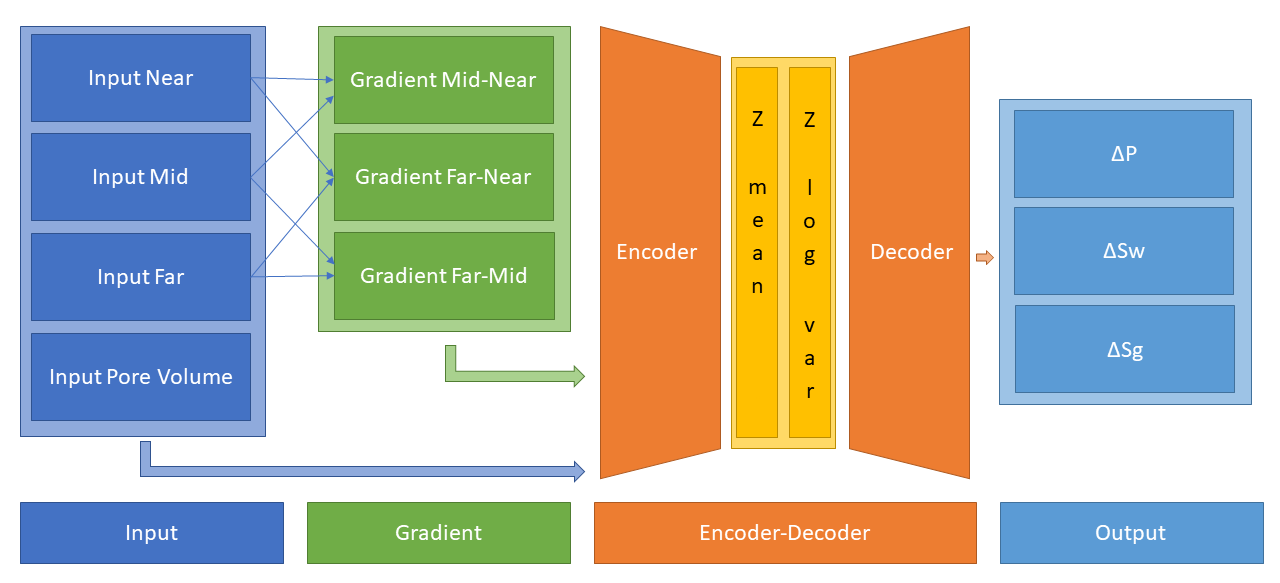
\includegraphics[width=\textwidth]{figures/AVO-Net.png}
    \caption{Architecture includes automatic physics-based gradient calculation of input seismic and an variational encoder-decoder architecture to invert seismic data for pressure and saturation changes \citep[from][]{dramsch2019including}}
    \label{fig:avo-net}
\end{figure}

Traditionally, 4D seismic \acf{qi} often relies on priors to reduce variance in the face of uncertainty. The inversion problem in this chapter is a pressure-saturation inversion from seismic amplitude difference maps in the Schiehallion field. The Schiehallion field is a stacked turbidite reservoir in the UK North Sea, which makes it very heterogeneous and compartmentalized. The T31 sandstone reservoir has the most lateral extent with the thickness ranging from 5~m to 30~m. The small thickness of the reservoir layer results in the entire reservoir being contained in a single trough of a seismic wavelet, which leads us to treat the network as a 2D map instead of a 3D problem. The data available consists of simulation and field data with several timesteps of seismic data in near-, mid-, and far-angle stacks, and pore volumes, as well as, pressure changes and saturation changes for water and gas from simulation.

In \citet{dramsch2019including} we present a novel network structure that explicitly includes AVO gradient calculation within the network as physical knowledge, shown in \cref{fig:avo-net}. The network architecture was chosen to follow an encoder-decoder architecture as a forcing function for information distillation. Additionally, the bottleneck layer implements a variational encoding layer to be less susceptible to noisy input. The network explicitly includes AVO gradient calculation in the network architecture, considering it is physical knowledge we know will stabilize pressure and saturation change separation. Including basic physics knowledge leads to the network learning residual information, essentially defining another forcing function for the networks learning process.

The initial phase was carried out on simulation data with a train test split, leaving a full 4D time step as validation set. \acl{nas} was applied to the network to determine depth and width of the architecture, using a \ac{tpe} hyper-parameter search \citep{bergstra2015hyperopt}. Afterwards, to transfer the network to field data, the input of the network was combined with additive Gaussian noise \citep{bishop1995training} to train the network for noisy field data input. This was a manual process of estimating good noise levels.
%\aclp{dnn} can learn these data-dependent priors from training data.

\begin{figure}
    \centering
    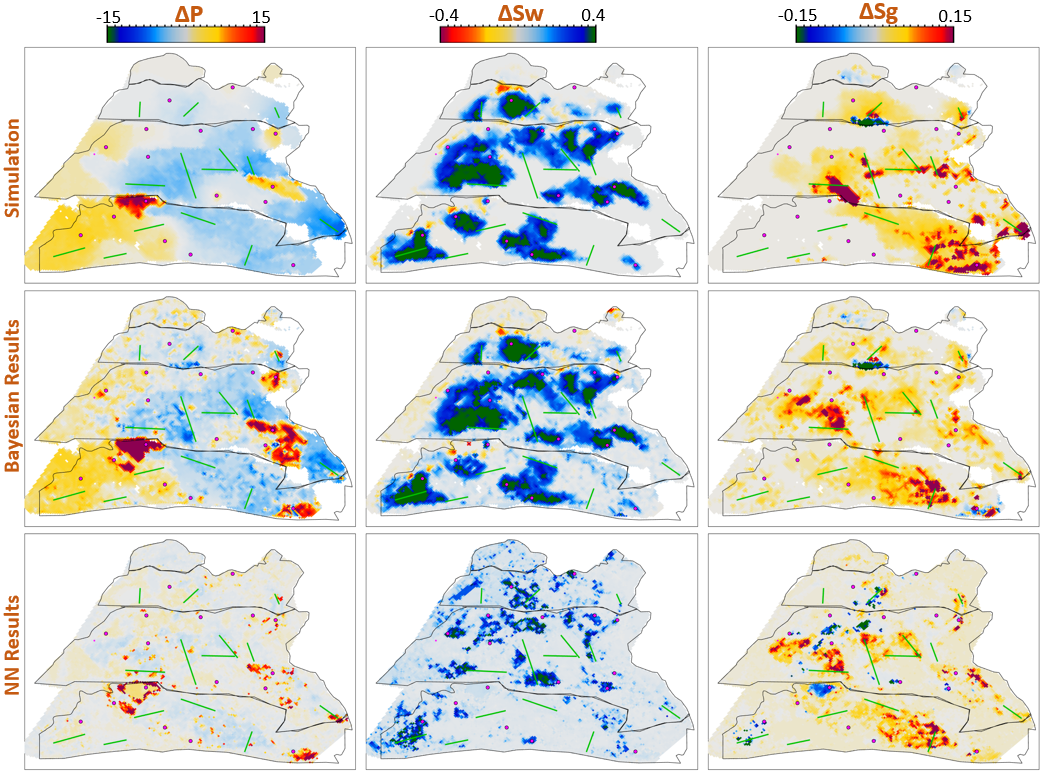
\includegraphics[width=\textwidth]{figures/NN_results.PNG}
    \caption{4D QI inversion results from Bayesian inversion and \acl{nn} inversion. Bayesian inversion closely resembles simulation output. \ac{nn} result showing good coherency, consistent amplitudes, but problems in strong changes of gas saturation \citep[from][]{dramsch2019deep}}
    \label{fig:avo-net-results}
\end{figure}

The workshop paper \citet{dramsch2019deep} contains these results compared to the simulation results and Bayesian inversion results, shown in \cref{fig:avo-net-results}. These initial results on limited training data show that the stochastic process can extract pressure saturation information from field data, after training on simulation data. While the overall result is promising, regions of strong gas saturation changes present a problem. This could be contingent problems in the modelling as well as the fact, that they generate strong amplitude differences and are far in between, essentially behaving like outliers. 

Learning meaningful information in deep neural networks is often contingent on interpreting the neural network. The results presented in \cref{fig:avo-net-results} contain three indicators that the network learned a meaningful inversion regression for the Schiehallion field. The network gets the overall trend in increase and decrease of pressure and saturation correct. Additionally, the range of output values for the network is unconstrained, but the network provides values in the ranges, that are expected from the simulation and Bayesian inversion results.  However, and more interestingly, the networks does not contain spatial information, being a feed-worward \ac{dnn} not a \ac{cnn}, yet returns continuous albeit noisy outputs when assembled into maps.

This chapter comprised of two workshop papers, shows a working implementation of a machine learning system inverting pressure-saturation data from seismic. Moreover, an implementation of a network trained on simulation data that is transferred to field data by noise modelling is presented. Finally, we show that including basic physics in the network architecture stabilizes training, making the case for physics-based \acl{ml}. Two journal papers are in preparation but not included in this thesis that analyze the network structure and the training data in detail \citep{corte2019exploring,dramsch2020physics}. 


% dramsch2019physics
% We present a novel neural network architecture that trains on synthetic data and provides insights into observed field seismic. The network explicitly includes AVO gradient calculation within the network as physical knowledge to stabilize pressure and saturation changes separation. We apply the method to Schiehallion field data and go on to compare the results to Bayesian inversion results. Despite not using convolutional neural networks for spatial information, we produce maps with good signal to noise ratio and coherency.

% dramsch2019deep
% Geoscience data often have to rely on strong priors in the face of uncertainty. Additionally, we often try to detect or model anomalous sparse data that can appear as an outlier in machine learning models. These are classic examples of imbalanced learning. Approaching these problems can benefit from including prior information from physics models or transforming data to a beneficial domain. We show an example of including physical information in the architecture of a neural network as prior information. We go on to present noise injection at training time to successfully transfer the network from synthetic data to field data.